\documentclass[a4paper,12pt]{report}

\usepackage[utf8]{inputenc} 
%\usepackage[margin=.5in]{geometry}  
\usepackage[portuguese]{babel} 
\usepackage{multirow}
\usepackage{graphicx}
\usepackage{caption}
\usepackage{subcaption}
\usepackage{mwe}
\usepackage{gensymb} %Degree º symbol
\usepackage{pdflscape} %landscape pages
\usepackage{amsmath}
\usepackage{verbatim}
\usepackage{amssymb}
\usepackage{setspace}
\usepackage{mathtools}
\usepackage{hyperref}
\usepackage{tikz}
\usepackage{float}  
\pagenumbering{arabic}

\usepackage{indentfirst} %\section or \chapter by default don't indent the first paragraph for some absurd reason!


%\singlespacing Para um espaçamento simples
%\onehalfspacing Para um espaçamento de 1,5
%\doublespacing Para um espaçamento duplo

\graphicspath{{images/}}


\begin{document}
	
	\begin{titlepage}
		\begin{center}
			
			\Large
			UNIVERSIDADE FEDERAL DE SANTA CATARINA\\
			EEL7051 - Materiais Elétricos\\
			\vspace*{5cm}
			\Huge
			\textbf{PROJETO PRÁTICO DE MATERIAIS ELÉTRICOS:}\\
			\textbf{TERMOPARES}
			
			\vspace{1.5cm}
			
			\vfill
			\Large
			\textbf{Alunos: Bobão 1}\\
			\textbf{Alunos: Bobão 2}\\
			\textbf{Alunos: Bobão 3}\\
			
			\textbf{Professor: Rambo} %Inserir nome completo do Rambo
			\vspace{0.8cm}
			
			Departamento de Engenharia Elétrica e Eletrônica\\
			Curso de Graduação em Engenharia Eletrônica\\
			Brasil\\
			
			
			
		\end{center}
	\end{titlepage}
	\Large
	
	\tableofcontents
	
	
	\pagebreak
	\listoffigures
	\pagebreak
	\tableofcontents
	\pagebreak
	
	\chapter{Introdução Teórica}
	
	Termopares são dispositivos formados pela junção de dois materiais condutores ou, por vezes, semicondutores, distintos, unidos em uma extremidade e sensíveis à variação de temperatura, expressando esta sensibilidade através de uma diferença de potencial. Possuem larga utilização industrial e em sistemas de instrumentação para aferição de temperatura, sendo o mais conhecido método para este tipo de medição.
	
	\noindent Um termopar é também conhecido por sua versatilidade como sensor de temperatura, portanto, normalmente são utilizados em uma ampla gama de aplicações - desde um termopar de uso industrial à um termopar regularmente encontrado em utilitários e aparelhos regulares. Devido à sua vasta gama de modelos e especificações técnicas, é extremamente importante entender a sua estrutura básica, como um termopar funciona, suas escalas para melhor determinar qual é o tipo certo e material do termopar para sua aplicação.
	
	\begin{figure}[htbp]
		\centering
		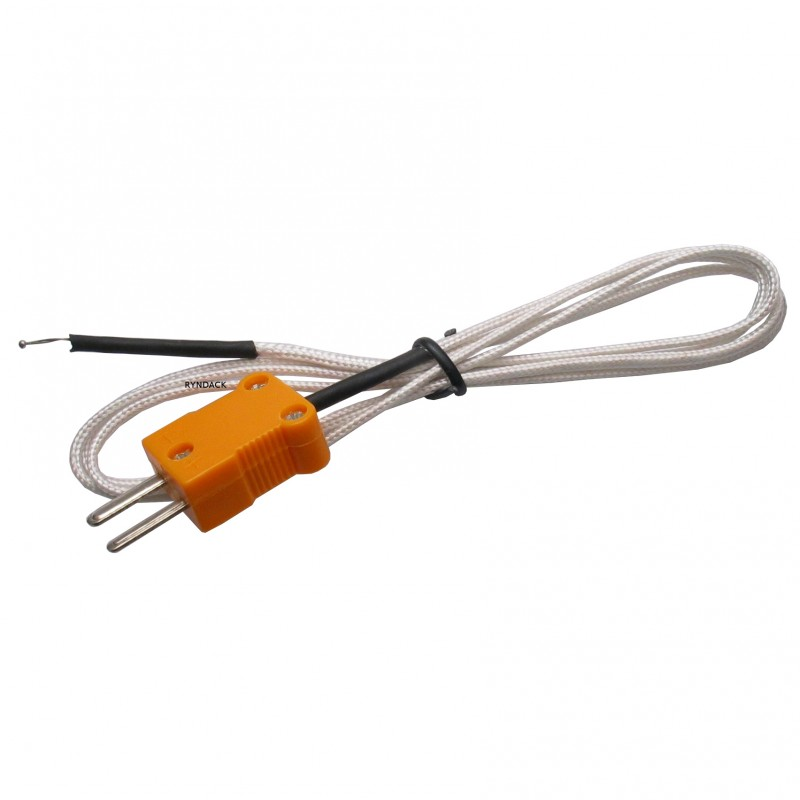
\includegraphics[scale=.2]{termopar-tipo-k-01.jpg}
		\caption{Termopar Tipo K}
		\label{real}
	\end{figure}
	
	\section{Utilização}
	Ao ser aplicada uma diferença de temperatura entre a junção de metais e as extremidades livres, haverá a geração de uma diferença de potencial da ordem de mV (milivolts) entre estas extremidades, da qual pode ser medida por um sistema de aquisição, utilizando-se comumente um multímetro como pode ser observado no esquemático da Figura \ref{esquematico}.
	
	\hfill \break
	\hfill \break
	
	\begin{figure}[htbp]
		\centering
		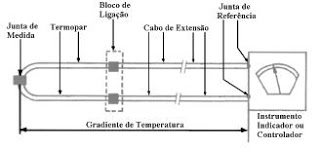
\includegraphics[scale=.8]{ABAAAAJ_sAG-68.jpg}
		\caption{Utilização do Termopar tipo K}
		\label{esquematico}
	\end{figure}
	
	\pagebreak
	
	\section{Efeito Seebeck}
	
	O princípio termoelétrico dos termopares deriva de uma propriedade física dos condutores metálicos, que quando  submetidos a um gradiente térmico em suas extremidades: a extremidade mais quente faz com que os elétrons dessa região tenham maior energia cinética e se acumulem no lado mais frio, gerando uma diferença de potencial elétrico entre as extremidades do condutor na ordem de alguns milivolts, como está representado na Figura \ref{seebeck}.
	
	\begin{figure}[htbp]
		\centering
		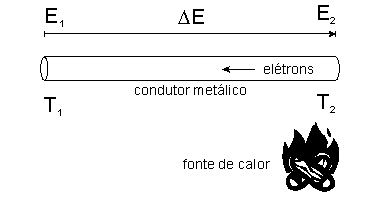
\includegraphics[scale=.8]{PrincipioTermoeletrico1.jpg}
		\caption{Efeito Seebeck}
		\label{seebeck}
	\end{figure}
	
	\noindent Podemos relacionar a temperatura com a força eletromotriz $\Delta E$ medido pelo coeficiente termodinâmico de Seebeck, representado na Equação \ref{seeback_eq}.
	
	\begin{equation}
	S = \frac{\Delta E}{\Delta T}
	\label{seeback_eq}
	\end{equation}  
	
	\noindent Quando dois condutores metálicos de natureza diferente são acoplados, na presença um gradiente de temperatura, os elétrons de um metal tendem a migrar de um condutor para outro, gerando uma diferença de potencial entre suas extremidades livres, como representado na Figura \ref{seebeck2}, de acordo com com seus coeficientes $S$, temos que a diferença de potencia gerada por essa diferença segue a Equação \ref{seeback_eq2}.
	
	\begin{figure}[htbp]
		\centering
		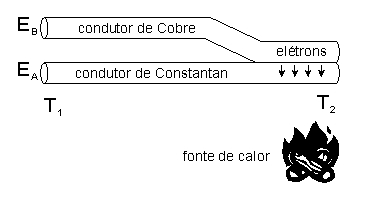
\includegraphics[scale=.8]{PrincipioTermoeletrico2.jpg}
		\caption{Efeito Seebeck para dois condutores diferentes}
		\label{seebeck2}
	\end{figure}
	
	\begin{equation}
	E = \int_{T_{1}}^{T_{2}} (S_{B}(T) - S_{A}(T))~\mathrm{d}T
	\label{seeback_eq2}
	\end{equation}
	
	\noindent Aproximando linearmente, para uma região de temperatura  onde os coeficientes possam ser considerados contantes podemos chegar na seguinte simplificação.
	
	\begin{equation}
	E = (S_{B} - S_{A}) \cdot  (T_{2} - T_{1})
	\end{equation}
	
	\noindent Podemos inclusive aplicando a equação \ref{densidade}, para assim determinar densidade termoelétrica do material.
	
	\begin{equation}
	J = \sigma (-\Delta V + E)
	\label{densidade}
	\end{equation}
	
	\noindent Onde $J$ é a densidade termoelétrica do material e $\sigma$ a condutividade do meio.
	
	\subsection{Efeito Peltier}
	O efeito Peltier se comporta de forma inversa ao efeito Seebeck, pois este efeito consiste consiste na produção de um gradiente de temperatura na junção de dois condutores de materiais diferentes quando submetidos a uma tensão elétrica em circuito fechado, como pode ser observado na Figura \ref{peltier} . 
	
	\begin{figure}[htbp]
		\centering
		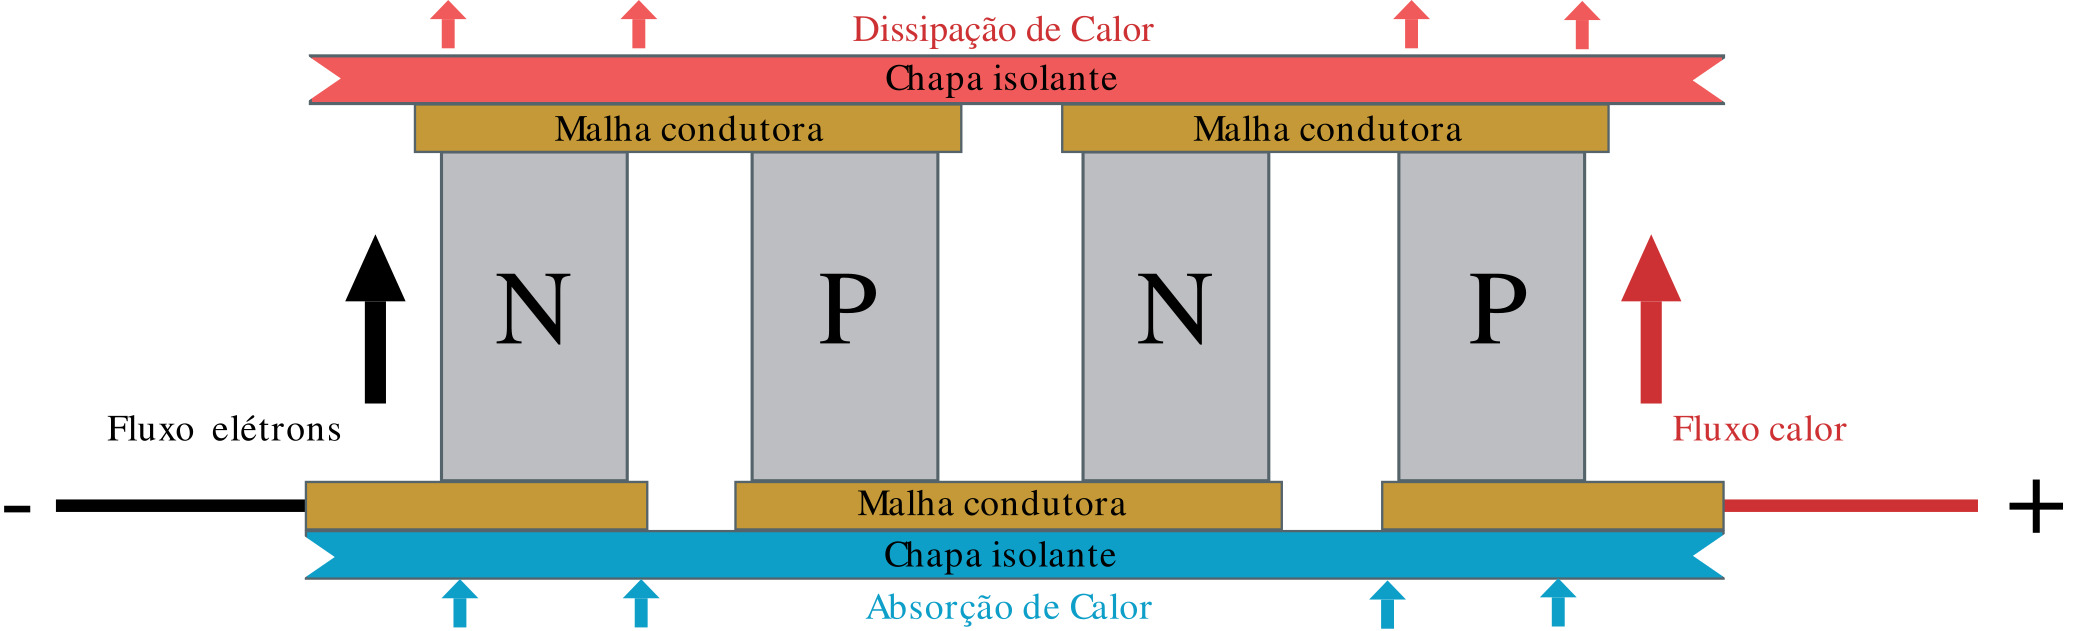
\includegraphics[scale=.8]{Esquema_Pastilha_de_Peltier.jpg}
		\caption{Funcionamento do Efeito Peltier}
		\label{peltier}
	\end{figure}
	
	\noindent A energia térmica do sistema é proporcional à corrente elétrica que percorre o sistema, sendo possível assim definir o calor associado pelo efeito pela Equação \ref{peltier_eq}.
	
	\begin{equation}
	Q_{p} = \Pi \cdot I
	\label{peltier_eq}
	\end{equation}
	
	\noindent Onde $Q_{p}$ é o calor associado, $\Pi$ o coeficiente de Peltier, e $I$ a corrente elétrica gerada pelo sistema. O coeficiente de Peltier esta relacionado com o coeficiente de Seebeck pela Equação \ref{peltier_eq2} e pela Equação \ref{peltier_eq3}.
	
	\begin{equation}
	\Pi = T \frac{S}{q}
	\label{peltier_eq2}
	\end{equation}
	
	\begin{equation}
	Q_{p} = S \cdot I \cdot T
	\label{peltier_eq3}
	\end{equation}
	
	\section{Efeito Thompson}
	
	O efeito Thompson, descreve a capacidade de uma corrente elétrica passando em um material no qual existe um gradiente de temperatura leva à produção de calor neste material, que atua em conjunto com o Efeito Joule, temos na Equação \ref{thompson_eq} o calor produzido por unidade de volume gerado por uma densidade de corrente $\overrightarrow{J}$.
	
	\begin{equation}
	Q = \rho J^{2} - \mu_{Th}\overrightarrow{J}\cdot \nabla_{r}T
	\label{thompson_eq}
	\end{equation}
	
	\noindent Onde $\rho$ é a resistividade do condutor e $\mu_{Th}$ o coeficiente de Thompson, podemos identificar a componente do Efeito Joule descrito por $\rho J^{2}$ e o segundo termo, o efeito Thompson que muda de sinal dependendo da direção de $\overrightarrow{J}$ sendo descritos como efeito positivo/negativo de Thompson para cada situação. E também vale ressaltar que o coeficiente de Thompson esta relacionado com o coeficiente termo-elétrico(S) pela Equação \ref{thompson_eq2}.
	
	\begin{equation}
	S = q \int_{0}^{T} \frac{\mu_{Th}}{T} \mathrm{d}T
	\label{thompson_eq2}
	\end{equation}
	
	\pagebreak
	
	\section{Aplicações}
	
	Termopares podem ser utilizados em equipamentos via medição de tensão, geralmente utilizando algum aspecto de instrumentação eletrônica. A partir da tensão mensurada, é possível calcular a temperatura utilizando métodos de \textit{look-up table} e interpolação. Com uma interpolação combinando métodos de segundo e terceiro é possível ter um erro mínimo para um bom \textit{range} de temperatura. 
	
	É possível, ainda, comprar designs analógicos e digitais de referência para instrumentação de termopares. Um exemplo é o design \texttt{TIDA-00468} da \textit{Texas Instruments\textsuperscript{TM}}, que oferece sensoriamento de -270\degree C até +1372\degree C para termopares do tipo K.
	
	A escolha do design é importante, visto que o custo agregado ao sensoriamento pode ser até maior que o custo do dispositivo em si, apesar do sensoriamento digital ser relativamente barato no presente momento.
	
	Na tabela a seguir é possível ver caraterísticas de operação de alguns tipos de termopares populares.
	
	\begin{landscape}
		
		\begin{center}
			\begin{tabular}{|c|c|c|c|c|c|}
				\hline 
				Type & Positive Material	 & Negative Material	 & Accuracy\footnote{De acordo com a Comissão Eletrotécnica Internacional 584-2}
				Class 2	 & Range \degree C
				(extension) \\ 
				\hline 
				B  & Pt, 30\%Rh	        & Pt, 6\% Rh                          & 0.5\% 800\degree C     & 50 to 1820 \\ 
				\hline 
				E  & Ni, 10\%Cr	        & Cu, 45\% Ni	                      & 0.5\% or 1.7\degree C  & -270 to 1000 \\ 
				\hline 
				J  & Fe                 & Cu, 45\% Ni	           			  & 0.75\% or 2.2\degree C & -210 to 1200 \\ 
				\hline 
				K  & Ni, 10\%Cr         & Ni, 2\% Al 2\% Mn 1\% Si            & 0.75\% or 2.2\degree C & -270 to 1372 \\ 
				\hline 
				N  & Ni, 14\%Cr 1.5\%Si & Ni, 4.5 \% Si 0.1\% Mg              & 0.75\% or 2.2\degree C & -270 to 1300 \\ 
				\hline 
				R  & Pt, 13\%Rh         & Pt                                  & 0.25\% or 1.5\degree C & -50 to 1768 \\ 
				\hline 
				S  & Pt, 10\%Rh	        & Pt                                  & 0.25\% or 1.5\degree C & -50 to 1768 \\ 
				\hline 
				T  & Cu                 & Cu, 45\% Ni                         & 0.75\% or 1.0\degree C & -270 to 400 \\ 
				\hline 
			\end{tabular} 
		\end{center}
	\end{landscape}
	Esses dispositivos podem ser divididos em dois grupos principais:
	
	\begin{itemize}
		\item Nobres: Contém ligas nobres na sua composição, como platina. Geralmente possuem uma temperatura mais alta de operaçã. Exemplos incluem os tipos R, S e B.
		\item Base: Mais comuns, geralmente feitos com ligas de níquel em um ou ambos materiais. Exemplos incluem os tipos J, K, T e E. O nome "base" vem do inglês "\textit{base metal}", denotando um metal relativamente barato, oposto aos metais preciosos.
	\end{itemize}
	
	\subsection{Construção}
	
	Tipos de termopares diferentes servem propósitos diferentes. Dentro dos tipos de junções, existem características de operação, e além disso, existem formas de construção que podem ser melhor utilizadas em algum ambientes específico. Questões como vibrações mecânicas, radiação ou operação Ininterrupta são considerações que devem ser realizadas ao escolher o tipo de termopar, e o próprio meio de instrumentação.
	
	Quatro tipos de construção do dispositivo em si podem ser encontradas:
	
	\begin{itemize}
		\item Aterrados: Os dois materiais são soldados juntamente com o invólucro. Permite respostas relativamente rápidas, porém pode apresentar um mau desempenho em aplicações com muita interferência eletromagnética.
		
		\item Não aterrados comum: Os dois materiais são isolados do invólucro por algum tipo de material. Mais estável que o Aterrado, porém tem um tempo de resposta significativamente mais lento.
		
		\item Expostos: A junção é totalmente exposta, sem invólucro. Melhor tempo de resposta, porém é extremamente susceptível a corrosão.
	\end{itemize}
	
	%gráficos equações----
	\section{Potência Termoelétrica}
	
	%equaçoes e gráficos ------
	\section{Leis Termoelétricas}
	
	Relações eletromagnéticas .....
	
	\section{Simulações}
	
	Simulações em Python ----
	
	\section{Conclusão}
	
	\section{Referências}
	\nocite{*}
	
	\bibliographystyle{IEEEtran}
	%\bibliography{Materiais}
	
\end{document}


